% ++++++++++++ Controller PSoC Master klassen ++++++++++++++
\subsubsection{Boundary-klasse: Distancesensor}

\begin{figure}[h]
\centering
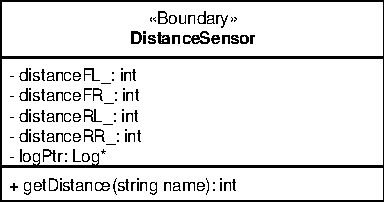
\includegraphics[]{../fig/diagrammer/bil/cd_distancesensor.pdf}
\caption{Klassebeskrivelse af boundary-klassen DistanceSensor}
\label{fig:cd_distancesensor}
\end{figure}

\textbf{Attributter}

\begin{table}[h]
\begin{tabularx}{\textwidth}{| Z | Z | L{10cm} |} \hline
Navn & Type & Beskrivelse \\\hline
\texttt{addrFL} & \texttt{int} &Adresse til forreste venstre afstandssensor.\\\hline
\texttt{addrFR} & \texttt{int} &Adresse til forreste højre afstandssensor.\\\hline
\texttt{addrRL} & \texttt{int} &Adresse til bagerste venstre afstandssensor.\\\hline
\texttt{addrRR} & \texttt{int} &Adresse til bagerste højre afstandssensor.\\\hline
\texttt{distanceFL} & \texttt{int} &Midlertidig variabel der indeholder afstanden fra forreste venstre afstandssensor.\\\hline
\texttt{distanceFR} & \texttt{int} &Midlertidig variabel der indeholder afstanden fra forreste højre afstandssensor.\\\hline
\texttt{distanceRL} & \texttt{int} &Midlertidig variabel der indeholder afstanden fra bagerste venstre afstandssensor.\\\hline
\texttt{distanceRR} & \texttt{int} &Midlertidig variabel der indeholder afstanden fra bagerste højre afstandssensor.\\\hline
\texttt{fd} & \texttt{int} &Variabel der anvendes som reference til i2c-bussen som sensorerne er tilkoblet\\\hline
\texttt{logEntry} & \texttt{string} &Variabel der indeholder reference til loggen.\\\hline
\end{tabularx}
\caption{Attributter for klassen DistanceSensor}
\label{table:attr_distancesensor}
\end{table}

\textbf{Metoder}

\begin{table}[h]
\begin{tabularx}{\textwidth}{| L{2.5 cm} | Z |} \hline
Prototype & \texttt{int getDistance(string name)} \\\hline
Parametre & \texttt{name} \newline Navnet på den sensor som der skal læses fra. Kan en af fire muligheder "FL", "FR", "RL" og "RR". \\\hline
Returværdi &  \texttt{int} \newline Afstanden for til nærmeste sensor for den pågældende sensor. Tallet er angivet i cm. \\\hline
Beskrivelse & Metoden læser afstanden som en afstandssensor befinder sig fra en forhindring. \\\hline
\end{tabularx}
\caption{Metodebeskrivelse for \texttt{getDistance}}
\label{table:met_getdistance}
\end{table}
\clearpage


Afstandssensorene leveres formonteret på chip hvor benene fra IC'en er trukket til harwinpins som let kan tilgås. Til kommunikationen benyttes følgende linjer: 

\begin{itemize}
	\item pin 7: VCC: Forsyning
	\item pin 6: GND: Reference
	\item pin 5: SCL: Clock
	\item pin 4: SDA: Data
	\item pin 3: Benyttes ikke
	\item pin 2: Status
	\item pin 1: Temp adresse 
\end{itemize}

Data kommunikeres på SDA-linjen med reference til clock'en. ''Status'' benyttes til at angive om sensoren er i gang med at performe en ''range reading''. 
Pin'en holdes højt så længe sensoren scanner, og trækkes lavt når operationen er fuldført og data kan leveres. Når pin'en er høj ignoreres al I2C-kommunikation.

For at initiere sensoren, ''Temp-adresse''-pin'en hvor der sendes en unik 7-bit adresse til sensoren.
   
Afstandssensorene benytter sig af I2C-bussen til kommunikation med Pi'en. Hertil benyttes I2C-tools biblioteket.
Dette bibliotek skal derfor hentes og aktiveres i linux-distrubutionen.

I2C device filer er CDD med major-nummer 89, og hver enkelt adaptor der er tilkoblet systemet får vedhæftet et minor-nummer, 
disse device filer findes i /dev/i2c-X, hvor X er et unik minor-nummer fra 0-256. Herfter er hver enkelt i2c-adaptor nu identificerbar og kan tilgås enkeltvis. 

Herefter skrives en klasse der kan håndtere de ønskede kald til de 4 afstandssensorer. 
I dette tilfælde ønskes der at implementere initDistance() og en getDistance() og i disse funktioner benyttes systemkald til at tilgå Hardwaren direkte, og aflæse de 4 sensorer via I2C-bussen.